%!TEX root = ../dokumentation.tex

\chapter{Evaluation}\label{cha:Evaluation}

\paragraph{Used example geometry and shaders}

For a basic example a scene consisting out of a tetrahedron which is rendered in three instances is chosen. These instances are assigned different color and different transformations as shown in  \autoref{fig:exampleScene}.

The example for a vertex shader is applying the instance transformation to the vertex position and to its normal, applying a camera transformation to the resulting position and passing through the instance color.

The example for the fragment shader receives the position, the normal and the instance color and applies a light calculation based on a given directional light and the camera position.

\begin{figure}[h!]
  \centering 
  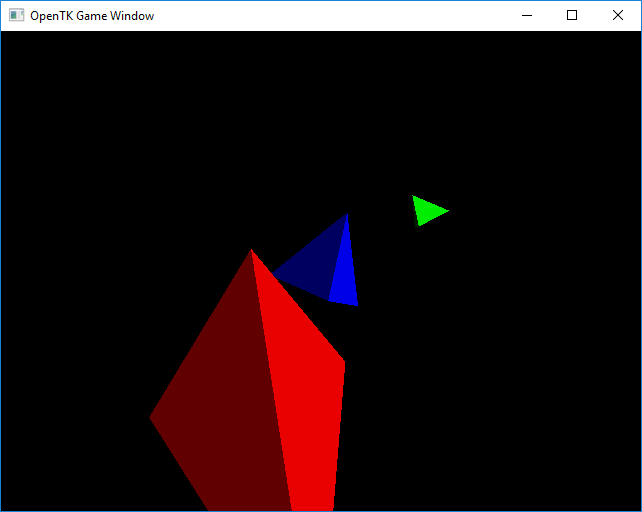
\includegraphics[scale=0.6]{scene.png}
  \caption[Screenshot of example scene of the project]{Project scene}
  \label{fig:exampleScene}
\end{figure}

\paragraph{Translation functionality}

For the chosen example shaders, all parts of the C\# shader code are translated to a functioning shader in GLSL. The code examples in \autoref{lst:sharpVertex},\autoref{lst:outputVertex}, \autoref{lst:sharpFragment} and \autoref{lst:outputFragment} show shaders written in C\# and their respecitve translation in GLSL. As seen in the vertex shader all parts of the C\# code have their equivalent in the shader code. For the fragment shader the result has a output variable for the color in addition to this. This additional output exists because this output is implemented in the base class for a fragment shader shown in \autoref{lst:fragmentBase}. In addition to the translation of the existing parts in the C\# code the headline for the version number is added for both shaders in the translation process. In the example this version number is always set as "version 430 core".

\begin{lstlisting}[caption = {Vertex shader written in C\#}, label = {lst:sharpVertex}]
class PassVertex : VertexShader
{
    [In]
    public Matrix4x4 InstanceTransformation { private get; set; }
    [In]
    public Vector3 Pos { private get; set; }
    [In]
    public Vector4 Color { private get; set; }
    [Out]
    public Vector4 Col { get; private set; }
    
    public override void Main()
    {
        Position = (InstanceTransformation * new Vector4(Pos, 1));
        Col = Color;
    }
}
\end{lstlisting}

\begin{lstlisting}[caption = {Vertex shader translated in GLSL}, label = {lst:outputVertex}]
#version 430 core
in mat4 InstanceTransformation;
in vec3 Pos;
in vec4 Color;
out vec4 Col;

void main()
{
        gl_Position = (InstanceTransformation * vec4(Pos, 1));
        Col = Color;
}
\end{lstlisting}

\newpage

\begin{lstlisting}[caption = {Base class of a fragment shader in C\#}, label = {lst:fragmentBase}]
public abstract class FragmentShader : Shader
{
    [Out]
    public Vector4 Color { get; protected set; }
}
\end{lstlisting}

\begin{lstlisting}[caption = {Fragment shader written in C\#}, label = {lst:sharpFragment}]
class PassFragment : FragmentShader
{
    [In]
    public Vector4 Col { private get; set; }
    
    public override void Main()
    {
        Color = Col;
    }
}
\end{lstlisting}

\begin{lstlisting}[caption = {Fragment shader translated in GLSL}, label = {lst:outputFragment}]
#version 430 core
out vec4 Color;
in vec4 Col;

void main()
{
        Color = Col;
}
\end{lstlisting}

\paragraph{Result of the simulation}

Running the translated GLSL shaders on the GPU with the example described above result in outputs that can't be distinguished as shown in \autoref{fig:translated} and \autoref{fig:simulated}.

\begin{figure}[h!]
    \centering
    \begin{minipage}{0.48\textwidth}
        \centering
        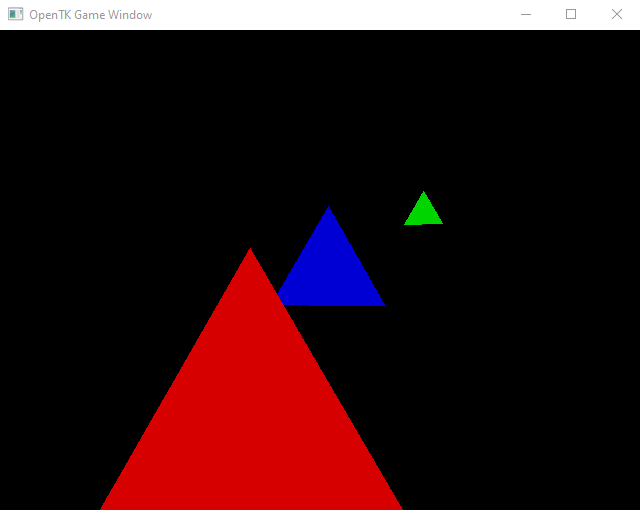
\includegraphics[width=1\textwidth]{translated.png} % first figure itself
        \caption[Screenshot of example scene rendered with translated shaders]{Result of rendering with the translated shaders}
        \label{fig:translated}
    \end{minipage}\hfill
    \begin{minipage}{0.48\textwidth}
        \centering
        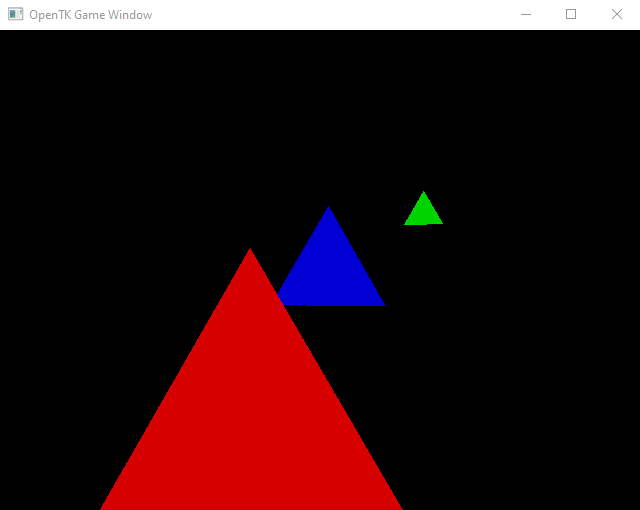
\includegraphics[width=1\textwidth]{simulated.png} % second figure itself
        \caption[Screenshot of example scene rendered with C\# shaders on simulated pipeline]{Result of rendering with the C\# shaders on simulated pipeline}
        \label{fig:simulated}
    \end{minipage}
\end{figure}

The only noticeable difference between rendering the translated shader in comparison to rendering the simulated version is the performance. As shown in \autoref{fig:perfCPU} rendering a single frame in the simulation on the CPU takes about 1500 ms while rendering a single frame on the GPU with the GLSL shaders takes only 0.0015 ms for this example. These values are gained while running the example on a Nvidia GTX970 as GPU and a Intel i7-6700K as CPU. But as described in \autoref{paragraph:objective} this is tolerable for the purpose of debugging.

\begin{figure}[h!]
    \centering
    \begin{minipage}{0.58\textwidth}
        \centering
        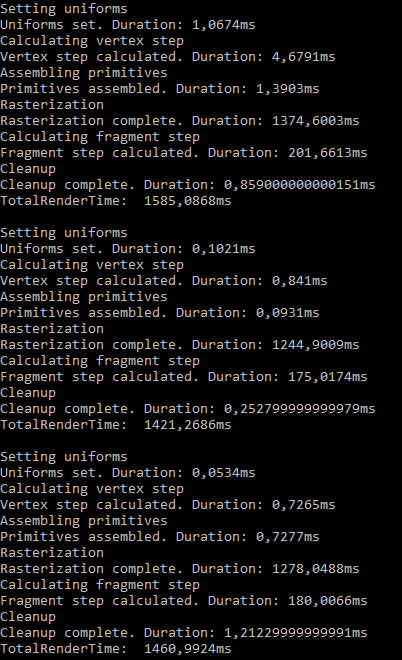
\includegraphics[width=1\textwidth]{performanceCPU.png} % first figure itself
        \caption[Screenshot of console output rendering the example with C\# shaders on simulated pipeline]{Permormance of rendering with the C\# shaders on simulated pipeline on CPU}
                \label{fig:perfCPU}
    \end{minipage}\hfill
    \begin{minipage}{0.38\textwidth}
        \centering
        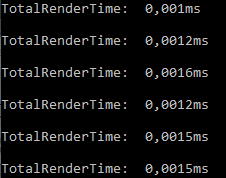
\includegraphics[width=1\textwidth]{performanceGPU.png} % second figure itself
        \caption[Screenshot of console output rendering the example with translated shaders]{Performance of rendering with the translated shaders on GPU}
        \label{fig:perfGPU}
    \end{minipage}
\end{figure}

\paragraph{Debugging of the C\# shaders}

The shaders written in C\# and running in the simulated graphics pipeline can be debugged as any other C\# code in VisualStudio.

It is possible to set breakpoints and add conditions to them. Setting such a condition could be used to debug a specific fragment or vertex. From these breakpoints it is possible to step through the code, inspect the variables and even navigating backwards through the call stack.

In the example no exceptions are thrown but if any of the underlying methods would throw a exception VisualStudio would stop the execution and show the problem in the debugger.

Most of the debugging tools listed above can be seen in \autoref{fig:debugging}

\begin{figure}[h!]
  \centering 
  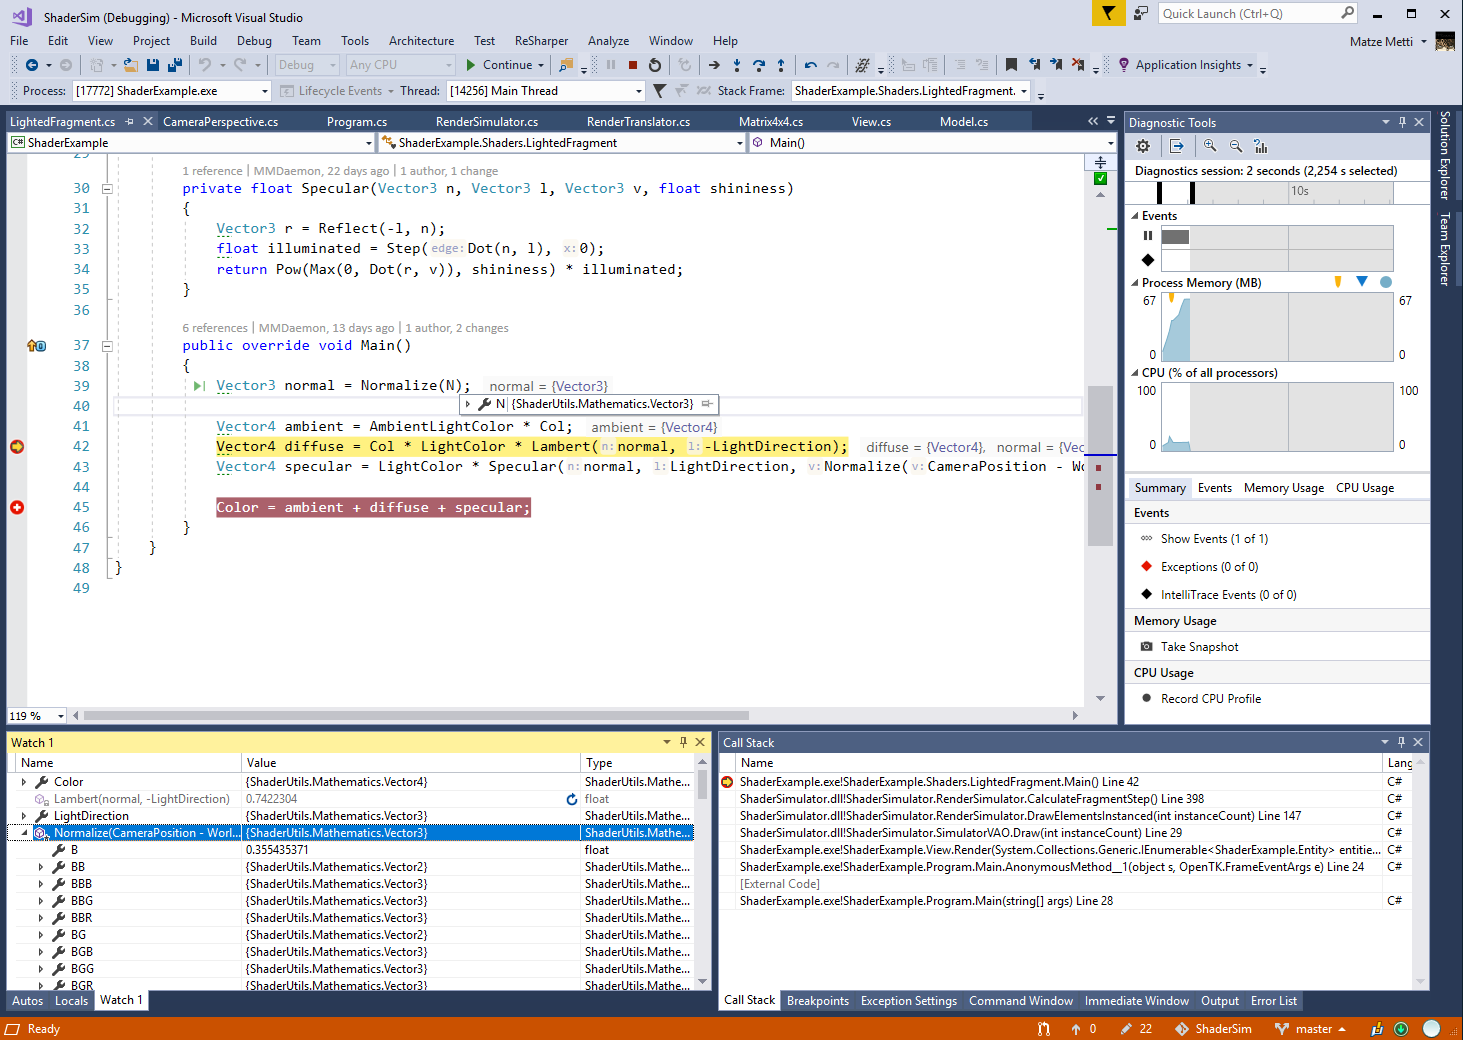
\includegraphics[angle=90,origin=c,width=1\textwidth]{debugging.png}
  \caption[Screenshot of debug screen within VisualStudio]{Debugging shader with different tools in VisualStudio: setting breakpoints, breakpoints with conditions, stepping through the code, variable inspection, navigating through the call stack}
  \label{fig:debugging}
\end{figure}

\paragraph{Behavior when using non supported features in the C\# shader}

If the code for a non supported method or value type would be written in the C\# shader code the program would not compile and neither the simulation nor the translation would start.

It would be possible to give the path of a file not used in the project as a shader to the translator. If this code would contain a C\# shader written in the correct syntax using methods of value types not supported in the example the translator would run and return a GLSL shader. The translator would simply keep the names of every method call and value type that is not defined by a "TranslationAttribute". If these kept names match the names of the methods and value types in GLSL the shader could be executed. If any of the names would not have a match in GLSL, the resulting code would not be compilable.